\section{Technology Assessment} % (fold)
\label{sec:technology_assessment}

According to the four types of prototypes in design science \cite{Johannesson:2014co}, our prototype was intended to be of the model type. A model can be used for supporting the construction of other prototypes, and hopefully our model can be reused by later projects. We wanted to come up with a proposed design that enabled us to test different aspects of using low energy sensors for wireless ECG monitoring, as well as how suitable the Bluetooth Smart protocol was as a medium for streaming raw ECG data. Based on what we knew from previous literature we decided the following three aspects constituted the baseline functional tests that would answer our research questions:
\begin{itemize}
	
	\item End to end latency
	\item Battery life
	\item Maximum throughput
  
\end{itemize}
\noindent
In order to validate our proposed design we decided to build a working prototype. Our prototype takes the form of a test bed that can be used to address the items listed above experimentally. This section starts with a discussion on different technical and architectural alternatives and the decisions made. Later we describe how it was implemented, before we evaluate the baseline functional tests.

\subsection{System architecture} % (fold)
\label{sub:system_architecture}

As mentioned in Section~\ref{sec:literature_review}, different architectures has been proposed and discussed in large by previous research. A general solution to how WBANs should be organized in relation to existing infrastructure do not exist, and is an important research topic. Mainly two different architectures have been discussed earlier: One where the WBAN routes all traffic through a personal gateway, and another one where it directs the traffic directly to an access point. See Figure~\ref{fig:architecture}. In \cite{Shahamabadi:2013df} a third approach is proposed. This merges the two former ones, where WBAN data is sent directly to the access point, while the personal gateway is given the responsibility of coordinating mobility issues like exchanging handover messages on behalf of the WBAN. In the following section, we will compare the first two approaches as seen in Figure~\ref{fig:architecture}.

\begin{figure}[H]
\centering
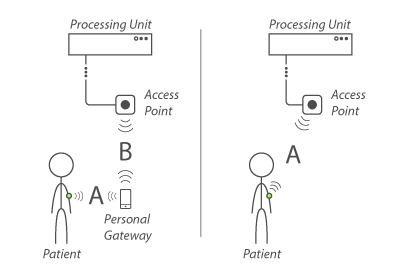
\includegraphics[scale=1]{img/figures/architecture.png}
\caption{Here A represents Bluetooth Smart while B is 802.11}
\label{fig:architecture}
\end{figure}

\noindent
Based on what we know about the existing telemetry systems deployed today and the research on WBAN sensor devices, it is improbable that all sensory devices will be (A) developed by the same manufacturer, and (B) that they all communicate over the same physical medium. The question of data interoperability is an interesting topic, because of the technical constraints imposed by the small sensors. At what point in the pipeline do we enforce the standardized data formats for exchanging medical information? In general, we believe this should be done as early as possible in the process, preferably at the node level. However, we want to highlight two arguments to why this might not be optimal: Although there has been invested a lot of effort by standardization organizations like HL7 and OpenEHR the last 30 years, data standardization in health care remains a challenge - not only across institutions, but also between information systems located at the same hospital. Based on this, requiring standardized formats with reduced footprint, optimized for constrained sensory devices, might not be realistic. As mentioned in Sect. 3, organizations like Continua are currently trying to bridge this gap, but with a primary focus on personal health technology, not clinical. This is a topic that need more research.

Another argument to why it might not be feasible to enforce todays standardized data formats for physiological measurements at node level, is related to the technical constraints of these devices. In order to keep the energy consumption down, overhead is reduced and as little data as possible is sent. This is especially true for continuous, streaming data sources like ECG. The approach Continua and ISO/IEEE has to this problem is to make smaller standardized measurement data formats tailored for constrained devices. Then they specify how these data formats should be transformed or mapped onto richer, data formats with a larger space footprint at a gateway level.

Relating this to the architectures discussed in previous research, we identify certain practical advantages of routing all traffic trough the personal gateway: Making a personal gateway compatible with a given sensor and its manufacturer specific or protocol specific\footnote{If standardized data formats are used} data format is a trivial task through software applications installed on the personal gateway device. The same triviality does not hold for a smart access point/boarder router wanting to transform the data into a richer, standardized data format. In a reality where a standardized data format is not implemented by every sensor node, giving an access point the role as a WBAN sink, as suggested by \cite{DrAmirMohammadRahmani:2014vx} seems highly impractical: All access points in a roaming environment would have to be compatible with custom data formats from several WBAN sensors carried by a multitude of patients. In this scenario, we only see smart gateways/access points being able to fulfill this data processing and transformation responsibility if standardized data formats for every physiological measurement is implemented at WBAN node level.

Based on these considerations, our proposed architecture consist of the following parts: a single sensor node simulating a patient ECG device, a personal mobile gateway acting as a WBAN sink to be carried by the patient, a monitoring server available on a local or remote network together with a client interface for remote monitoring. In order to reduce the scope and complexity we have decided to only include one node in our prototype. This is a clear limitation with our prototype and study, as we only consider a single-hop network topology in instead of a mesh topology, which is proven to be the most effective topology for WBANs. One concern here might be that Bluetooth does not currently support mesh networks, but as as Feb. 24 2015 the Bluetooth SIG formally announced formation of the Bluetooth Smart Mesh Working Group \cite{bt:sig:mesh}, and we operate under the assumption that this will be supported in future versions. The gateway should have the responsibility of routing the sampled data from the WBAN to an external endpoint. In accordance with Continua's guidelines, we also propose that the gateway enforce interoperability by transforming the data into a standardized medical format. Later in this section we propose a suitable  standardized data format. See Table~\ref{tab:system_components} for a formal description of each component of our prototype.

% TODO create table system_components

An overview of the different prototype components:
\begin{itemize}

  \item[\textbf{Node:}] A node is the sensory device that does one or more physiological measurements and communicates it wirelessly to either another node or to a sink in the WBAN. In order to achieve wearability the nodes has to be as small as possible. Batteries are often the largest part of today’s sensory nodes and the biggest energy consumer is typically the antenna \cite{Ullah:2010ci}.

  % \item[\textbf{WBAN:}] Multiple nodes connected together constitute the wireless body area network (WBAN). The network topology of these vary depending on the communication protocol between the nodes, but they are typically organized as single hop stars, or multi-hop mesh networks \cite{Anonymous:6F6UBBK9}. Desirable qualities in a WBAN is a low energy PHY layer, and a flexible MAC protocol capable of doing smart routing and the ability to be self organizing \cite{Anonymous:XKViPHhV} \cite{Anonymous:OEjzuKTe}.

  \item[\textbf{Personal gateway:}] In previous literature this tier in the patient monitoring stack is also called a Personal Server (PS) or a WBAN sink. This can be a touch device with a graphical user interface, a tele health station, or just a dedicated sink in the WBAN with a larger battery. Because of the low energy consumption of the nodes, you typically need to facilitate communication between the WBAN and a boarder router with some device that has more battery capacity, a stronger antenna and that is easier to replace on a frequent basis. For the remainder of this thesis we will assume the personal gateway is a feature rich touch device, with a graphical user interface like the Samsung Galaxy S6.

  % \item[\textbf{Boarder router:}] The border router can be categorized as a end node in a local area network providing access network access for proprietary devices through one or more wireless networking interfaces. Based on the network configuration and overall architecture of the monitoring system this router may have different responsibilities. A smart-gateway can for example provide additional services specialized for sensory data. These services can include but are not limited to local caching, pre-processing and on-demand-processing, WBAN discovery, localization and more \cite{DrAmirMohammadRahmani:2014vx}.

  \item[\textbf{HIS:}] Hospital information system. This is a common term for the various types of information systems at hospitals. The way these are implemented and used varies from across borders, regions, and even between different departments within the same hospital. Because of this invariance in systems and practice, interoperability across communication protocols and data formats is of outmost importance. For the remainder of this thesis we will discuss only one HIS, namely the monitoring central. This is responsible for collecting, processing and storing and serving sensor data to clients.

\end{itemize}

% subsection system_architecture (end)

\subsection{SoC Considerations} % (fold)
\label{sub:soc_considerations}

While deciding on what platform to use for our proposed design we looked through a wide array of different System on a Chip (SoC) solutions and boards enabling rapid prototyping and testing with Bluetooth Low Energy and physiological metrics. In order to increase reproducibility and ease later projects, this sections contain an overview over the different boards we considered, together with strengths and weaknesses.

RedBears Nano \cite{newRef:36} development boards were of particularly interesting because of their form factor. They are based on the Nordic NRF51822 chip and measure only 18.5mmx21.0mm. However, we because our goal was not related to mobility the actual size of the chip was not important to us. Another board of interest was Bitalino's development board for capturing body signals \cite{newRef:37}. Among other things, it comes with interfaces and built in analog to digital converter for ECG leads. This could have been a good starting point for our prototype, but the development kit only supports Bluetooth 2.0 which was of little interest to us.

We looked at Zolertia \cite{newRef:38} development boards, and even ran some preliminary tests using simulated Zolertia Z1 motes and the Contiki Cooja Simulator. However, these are based on the 802.15.4 specification, and was therefore outside the scope of this project. The same accounts for the Tmote Sky \cite{newRef:39}, which have been used extensively in earlier research \cite{Milenkovic:2006er, Owner:2006ub, ChulsungPark:2006tf, SteveWarren:2005ws, ChulsungPark:2006tf, Anonymous:GyP6wjY5}

Among more medical targeted development kits we looked at Shimmer Tools \cite{newRef:41} which offer professional, medical grade wireless sensors suited for ``academic, applied and clinical researchers''. These were of particular interest because of the configurable ECG options and that it shipped with libraries \cite{newRef:41} for streaming and parsing data on the Android platform. However, the Bluetooth module used for wireless transmission is based on the RN-42 chip \cite{newRef:43}, which only supports the 2.1 version of the Bluetooth protocol. Another, similar development kit targeting clinical trials, research and teaching labs, is the BioRadio from Great Lakes NeuroTechnologies \cite{newRef:44}. This is a highly configurable device with both adjustable sampling rate (250Hz-16kHz) and sample resolution (12-24 bit), as well as a SDK for pc \cite{newRef:45}. To our knowledge the BioRadio has a newer Bluetooth chip supporting version 4.0. However, because of the high sample rate and resolution, it is highly unlikely that they utilize the low energy features of the specification, due to the bandwidth constraints of the low energy specification. A further discussion on Bluetooth bandwidth versus the minimum requirements for ECG can be found in Sect. 3. It is also unlikely that the firmware is customizable in commercial products like the ShimmerTools and BioRadio, and was these two devices was therefore not interesting to us.

After investigating these different development platforms, we decided to avoid development kits capturing real physiological data (Bitalino, ShimmerTools and BioRadio) for the sake of testability and reproducibility. This way it would be easier to conduct consistent experiments. However, these devices offer a great deal of functionality and possibilities both in terms of hardware capabilities, technical specifications and ease of development, and should be considered in later research.

Texas Instruments another major actor in the embedded community. They design and develop a wide array of semiconductors and hardware for industries ranging from audio and hifi to medical devices \cite{newRef:46}. In fact they have a own sensory product line for biological signals. TI also has an active research community publishing reference designs for various applications branded under the name TIDesigns \cite{newRef:47}. In the later stages of this project, we became aware of an for a 5-lead ECG monitor based on Bluetooth Low Energy \cite{Anonymous:Q0qkTQkl}. The existence of this reference design have not influenced neither our design choices nor research questions, as it was discovered late in the project. An overview of the TI's proposed design and the implications an earlier discovery of this reference design could have had are discussed in Sect. 6.

Most of the relevant development kits we evaluated were based on one of the Nordic nRF51-series chips \cite{newRef:36, newRef:36:2}. Because hardware design and development was uncharted territory for the researchers, the availability of online communities and documentation was a critical factor when assessing/deciding on what development kit to base our prototype on. Nordic themselves has a thriving community on their Stack Overflow inspired developer zone \cite{newRef:50}, which has at the time of writing has over 13,800 questions asked. Because of this we decided a development kit based on the  nRF51822 chip was our best alternative. Because Nordic Semiconductor also offer their own development kits, we decided to use those as the basis of our prototype, reducing the number of external dependencies. 

In terms of software development on these different boards, we investigated the different IoT operating systems and assessed the feasibility of using these for our purpose. After a quick survey, the small RiotOS \cite{Anonymous:a1din1ZK}, running on only 1.5kB RAM and 5kB of ROM, looked like the most promising alternative. A comparison of the major operating systems for IoT-applications can be found at \cite{Anonymous:a1din1ZK}. For our project however, it was concluded that the node functionality would be limited and specialized rather than general. Hence, adding a dedicated operating system to our already growing technology stack would impose more risk to our project. It should also be mentioned that this technology and the platforms that are being built around them are not very mature: The seeds for RiotOS were planted less than 10 years ago as it started out as an operating system for wireless sensor networks in Germany in 2008 \cite{newRef:52}. An example of this lack of maturity, is that we have yet to find a RiotOS library for accessing the Bluetooth stack on nRF51822 trough SoftDevices.

Due to the increasing risk and complexity more dependencies add to the development, we dropped support for 6LoWPAN, although this is an important advance for network interoperability in low energy devices. There was an interest for this when we started the project, but a concurrent research project investigating the practical limitations of using IPv6 enabled Bluetooth Smart (6LoWPAN) technology, was already in progress at the Department of Telematics.

% subsection soc_considerations (end)

\subsection{Node} % (fold)
\label{sub:node}

The first prototype iteration used a Nordic nRF51 evaluation kit from 2013, which supported Bluetooth Smart version 4.0 trough a software stack Nordic calls SoftDevices. A SoftDevice is a precompiled and linked binary that implements the Bluetooth protocol stack for NRF51 boards. Because of the board's relative old age (development in this area happens at a rapid pace) the latest Nordic SDK\footnote{The Nordic nRF5 SDK forms the foundation of what you need of drivers, libraries SoftDevices and code examples to develop your own low-energy Bluetooth, ANT product} support for this board was version 6, while the most recent SDK is at version 10. This turned out to cause a lot of compatibility problems, and the development process was tedious: We had to flash both SoftDevice and our own compiled software onto the board manually using Segger's J-Link software. In addition to this, the J-Link debugging options were not supported on our development system.

Because of the compatibility/legacy issues we had with the node in our initial prototype, we decided to replace the 2013 evaluation kit for a nRF51 Development Kit originally released late 2014 \cite{newRef:53}. This board supports a newer SDK (version 8), two new SoftDevices and ARM's mBED development platform \cite{newRef:54} The latter was crucial as it drastically eased the process of compiling and installing software on the development board. mBED is a online development platform for embedded devices developed and maintained by Arm \cite{newRef:55} along with partners and contributors. It solves the problem of setting up an correct environment for compiling C++ code specific to a given development board, by building and compiling programs in the cloud. This means they maintain and keep track of all dependencies and environment configurations needed for correctly building and compiling code specific to a given board before making a binary file available for download. An mBED enabled board connected to your computer via USB will be available as a mass storage device. In order to install the software, you simply drag the bundled binaries over to the mass storage device, and the software will auto-install. 

While the development process was eased, programming ARM Cortex M is still complicated, and so is Bluetooth Low Energy. Simulating ECG data is also a non-trivial task, and based on these three factors we decided to use as much available code for the board programming as possible.

In order to simulate the ECG data stream on the board, different existing ECG simulators written in C++ were considered \cite{newRef:56, newRef:56:1, newRef:56:2}. We decided to go for ECGSYN, a realistic ECG waveform generator created at Oxford and MIT \cite{newRef:56:2}. This is a flexible program that let us customize sampling frequency and mean heart rate among other things. ECGSYN generates a synthesized ECG signal based on algorithms described in \cite{newRef:58}. Se figure Listing~\ref{lst:ecgsyn:terminal} for an overview of the different adjustable parameters.

\begin{lstlisting}[caption={ECGSYN Commando Line Interface (CLI)}, label={lst:ecgsyn_terminal}, basicstyle=\tiny]

    >> ecgsyn $
    ECGSYN: A program for generating a realistic synthetic ECG
    Copyright (c) 2003 by Patrick McSharry & Gari Clifford. All rights reserved.
     
    O Name of output data file                 "ecgsyn.dat"
    n Approximate number of heart beats        256
    s ECG sampling frequency [Hz]              256
    S Internal Sampling frequency [Hz]         256
    a Amplitude of additive uniform noise [mV] 0
    h Heart rate mean [bpm]                    60
    H Heart rate standard deviation [bpm]      1
    f Low frequency [Hz]                       0.1
    F High frequency [Hz]                      0.25
    v Low frequency standard deviation [Hz]    0.01
    V High frequency standard deviation [Hz]   0.01
    q LF/HF ratio                              0.5
    R Seed                                     1
    (Type ? for Help)
    ->

\end{lstlisting}

\subsubsection{Maximum Throughput} % (fold)
\label{ssub:maximum_throughput}

Because experience with embedded software development was limited, we did some preliminary research on max throughput on Bluetooth Smart, before starting the customization and implementation of the ECGYN software on the development board. As mentioned in Section~\ref{sec:literature_review}, Bluetooth Smart specifies the theoretical max throughput to be 1 Mbit/s. However there are always factors limiting this theoretical capacity. In the following section will elaborate on these limiting factors, and comparing our findings with the minimum requirements of clinical ECG.

Note that in the following section, the mobile gateway acts the role of the client, and the wireless sensor acts the role of the server - the one with data. Once a Bluetooth Smart connection is established between two devices, the connection parameters \cite{newRef:59} control the frequency at which data can be sent between the two devices. The two connection parameters of interest to us are, minimum and maximum connection interval, which specify the minimum and maximum rate at which the client will ask for data from the server. By the specification, both fields have an allowed minimum and maximum value of 6 and 3200. By multiplying these values by 1.25ms we get the highest and the lowest frequency at which a central may ask for data: 7,5ms and 4s (4000ms).

The GATT protocol specifies different commands for the client to get information about the server. Among these, GATT offers notifications and indications. In high-throughput applications a client can request/register a notification on a given characteristic. This means that the server will send a notification containing maximum 20 Byte of user data to the client whenever data becomes available. These notifications are buffered by the SoftDevice and ACK-ed in the link layer. The Bluetooth specification allows for up to 6 packets to be sent per connection interval, but this number may vary between different implementations. This gives the following formula for calculating max throughput:

\[
\frac{1000\: ms/s}{CI}\: \times\: PPI\: \times\: BPP\: \times\: 8\: bits/byte = Throughput
\]

\newline
\noindent
Here, $CI$ is connection interval, $PPI$ is packets per interval, and $BPP$ represents the number of bytes sent per packet. Because packets per interval and the bytes per packet may vary between devices and operating systems, the maximum throughput over a Bluetooth Low Energy link is relative. However, maximizing the allowed values above, we get the following result: 

\[
\frac{1000\: ms/s}{7,5ms}\: \times\: 6\: packets\: \times\: 20\:bytes/packet\: \times\: 8\: bits/byte = 128\:Kbit/s
\]
\newline
\noindent
This is substantially lower than the advertised 1Mbit/s. In Table~\ref{tab:ble_device_throughput}  we present calculated throughputs for different devices based on their implementation of the Bluetooth specification. In Table~\ref{tab:ecg_sampling_rate} we list different configurations for capturing ECG with the minimum recommended sampling rates from \cite{Anonymous:j4z9MACD}. Generally, we see from this that low energy Bluetooth \textit{at the moment} is not well suited for clinical ECG due to it's restricted and variable throughput.

To confirm this discovery we tried installing some firmware \cite{nordic:throughputtest} to see if we indeed could achieve the 128 Kbps throughput. However, our LG G4 test device did not support the low connection interval, and dropped the connection as soon as the throughput test started. This proves that there are differences between different Android devices, as the operating system should support the optimal configuration.

% subsubsection maximum_throughput (end)

% subsection node (end)

\subsection{Gateway} % (fold)
\label{sub:gateway}

% TODO Create figure: throughput_overview from excel sheet

Although creating a user friendly application was not part of the scope of this project, we believe some thoughts on usability and context should be put into the creation of any artifact. We did not want to hard code the UUID address of Nordic chip into the gateway and connecting the data stream with a static endpoint address. Therefore we have created what we consider to be the bare minimum of a personal WBAN gateway user interface. The functional requirements of this user interface can be found in Table~\ref{tab:gatewayRequirements}.

\begin{table}[]
\centering
\caption{Personal Gateway Functional Requirements}
\label{tab:gatewayRequirements}
\begin{tabular}{|l|l|l|}
\hline
\textbf{FR\#} & \multicolumn{1}{c|}{\textbf{Description}} & \multicolumn{1}{c|}{\textbf{Priority}} \\ \hline
1             & Add new sensor                            & High                                   \\ \hline
1.1           & \ \ \ \ Scan for nearby BLE devices               & High                                   \\ \hline
1.2           & \ \ \ \ Select endpoint                           & High                                   \\ \hline
1.3           & \ \ \ \ Select BLE Characteristic                 & Medium                                 \\ \hline
1.4           & \ \ \ \ Add new endpoints                         & Low                                 \\ \hline
1.5           & \ \ \ \ Give each sensor a name                   & Low                                    \\ \hline
2             & Ability to test sensor connection         & Medium                                 \\ \hline
3             & Ability  to test endpoint connection      & Medium                                 \\ \hline
4             & List all sensor nodes                     & Low                                    \\ \hline
\end{tabular}
\end{table}

With an architecture dependent on a personal mobile gateway we chose a technology that was in accordance with our mission statement: available and open. The Android platform is not only more open than it's counterparts, but also supports higher throughput as seen in Table~\ref{tab:throughput_overview}.
The gateway would ideally be a multi-purpose touch device with a rich user interface, enabling an easy and practical way of setting up and configuring the wireless sensors a patient would be equipped with. Although outside the scope of this project, some thought have gone into the practicalities of setting up and managing a network of wireless sensor nodes. For further research we recommend looking into using Near Field Communication (NFC) technology for physically conducting events such as \emph{(A)} pairing sensors, \emph{(B)} connecting the gateway to the WBAN and \emph{(C)} authenticating medical professionals and patients on the personal gateway. We believe these are all use cases where an active NFC chip could drastically improve the user experience, but the subject need more research.

In the following section we will describe how we approached the implementation of the gateway application. Because we only intended to make a prototype, some details will be kept out for brevity. 

\subsubsection{User interface} % (fold)
\label{ssub:the_user_interface}

The functional requirements were prioritized and we developed the user interface in a iterative fashion as more functionality gradually were added. The resulting user interface is not user tested as this was outside the scope of this project. The ``front-end'' of the application consist of two simple views, as seen in Figure~\ref{fig:android_frontend}. As the application is opened the user is presented with a list of sensors connected to the gateway. Clicking either a sensor or the plus sign in the downright corner brings the user to the next screen, where you can either modify the existing device or add a new one. 

The application has prioritized functionality over reliability, but still some basic error handling and connection tests are implemented. Both when connecting to a Bluetooth Smart sensor and when selecting endpoint, the application tests the connection. How this is implemented is described in Section~\ref{ssub:bluetooth_module} and \ref{ssub:endpoint_module}. When both sensor and endpoint is selected, the user is able to activate the routing of the data by clicking on activate. The user would then be navigated back to the overview of previously added devices.

In terms of the interoperability issues mentioned in \ref{sub:system_architecture} we imagine the gateway application could be extended with a an online repository containing a growing amount of sensor peripherals as well as standardized data formats the data streams could be transformed into. These settings would be downloaded and stored together with the sensor node settings. Making the gateway application compliant with a wide array of proprietary sensors and compliant data formats.

% subsubsection the_user_interface (end)

\subsubsection{Bluetooth Module} % (fold)
\label{ssub:bluetooth_module}

We have split the Bluetooth functionality out in a separate and isolated part of the program. Depending on the hardware, a future version of the application could replace the Bluetooth module with, say a Zigbee interface.

% subsubsection bluetooth_module (end)

\subsubsection{Endpoint module} % (fold)
\label{ssub:endpoint_module}

% subsubsection endpoint_module (end)

% (I intend to cover the following aspects of the gateway software:)

% TODO insert Figure~\ref{fig:architectureWorkflow} 

% node -> bluetooth le -> android gateway -> websockets -> meteor webserver -> socket -> mongoDB -> 

% subsection gateway (end)

\subsection{Server} % (fold)
\label{sub:server}

Inspired by \cite{Thelen:2014ew} and informed of the development within the standardization communities like (HL7 FHIR), we decided to mock up a monitoring central using web technologies. In addition to vastly simplify product development for a manufacturer, using web technologies also enables rapid prototyping for small research teams with little resources. As seen in Figure~\ref{fig:serverRequirements} functional requirements of the server prototype was limited. Based on experience with similar technology we decided to write the server software in Javascript. Contrary to it's young age, this is a programming language that has matured a lot over the last couple of years, and is today the most popular technology for full-stack developers \cite{so:survey:results}.

Because of the simple requirements and limited timespan available building the monitoring server, it was decided to utilize a development platform built on Javascript. Meteor \cite{meteor} is an open source platform for web, mobile and desktop that satisfied our needs. It comes with database support (MongoDB) out of the box, and its own data managing layer. This layer is based on a protocol they call Distributed Data Protocol (DDP), which uses WebSockets as a lower layer message transport. DDP implements the publish-subscribe messaging pattern, which lets clients publish and subscribe to data collections over WebSockets \cite{ddp:github}. This functionality was ideal for this project as it made us set an endpoint for the gateway to publish the data coming from the sensor in short time. It should be noted that WebSockets make use of TCP at the transport layer. Alensanco and Garcia concluded TCP was not suitable for real-time ECG transmission in a wide area network \cite{Alesanco:2010kc}. They suggested UDP as a more suitable transport layer protocol, but they were transmitting data over a 3G network. Out prototype is connected to local area network over a WiFi link, offering substantial network speeds over telecommunication networks.

In accordance with use case \textsc{UC2.2}, we designed and implemented a client interface for medical professionals to access the ECG data streams. Technically speaking, the client view is served by the Meteor server and connected to the backend through a web socket connection. This allows for reactive data sources, meaning data flow back and forth between clients and the monitoring server seamlessly as it changes. In the client we have been looking at various ways of rendering the stream of values into an ECG plot. In the planning phase we landed on using a \texttt{jke-d3-ecg} \cite{jke:d3}, an open source chart component for the popular \texttt{D3.js} library drawing charts using Javascript. Note that this would not produce a clinical grade ECG plot, and was mainly considered for demonstrating purposes. When we implemented this, the bandwidth restrictions in the Bluetooth protocol was already discovered. As we did not have a stream of ECG values available from the sensor, we did not spend time implementing any plotting features. 

Because of Meteor's feature rich platform, our prototype has support for user accounts and easy patient management features such as the ability to subscribe to patient streams independently of one another. However, these features are not relevant for this project, and their implementation will not be discussed.

% subsection server (end)

\subsection{Evaluation} % (fold)
\label{sub:evaluation}

Because of inconsistencies and missing information in previous research, we wanted to conduct a series of tests that could validate our technology choices. Because of obvious limitations in our ability to perform some of these experiments traditionally, they have been designed to give us some indications on how the technology performs in practice. Therefore the experiments are linked to the use cases. 

Originally we had several other experiments as well, but these were removed in order to reduce the scope. 

\begin{itemize}
	\item End to end latency
	\item Battery life
	\item Maximum throughput
\end{itemize}
\noindent
Because of the discoveries made during the development of the prototype, maximum throughput and battery lifetime has not been addressed experimentally, but are rather discussed.

\subsubsection{End to end latency} % (fold)
\label{ssub:end_to_end_latency}

In order to get a baseline indication on the overall network performance of our prototype we set up an experiment measuring the end-to-end latency/delay. We were only interested in the $\Delta$ between the node and the client (the two endpoints) and not the intermediate steps. Because of this we were able to set up an experiment on our prototype where we synchronize the sending between the node and client. The goal for this experiment was to compare our delay with the maximum comfortable delay found in \cite{Alesanco:2010kc}, through clinical studies.
\\
\\
\noindent
\textbf{Hypothesis:} The transmission delay is marginal, even on a public area network with variable traffic.
\\
\\
\noindent
\textbf{Method:} We set up the node with software to send a application-layer message containing two control counters in a controlled interval. One acted as a global counter counting the total number of messages sent, the other one always started at zero and was incremented at each stop in the prototype pipeline: in the gateway, the server and the client. In order to synchronize the sending interval, the node was connected directly to the client over an USB interface. When sending the message to the gateway over Bluetooth, the node would also send a trigger pulse to the client over the UART protocol. See Figure~\ref{fig:transmission_delay_figure} for an overview of the setup. The client would receive this trigger pulse and make a timestamp indicating that the transmission has begun. When the client receives the message it makes another timestamp and calculates $\Delta$ along with checking the control counters to see if any messages have been lost during transmission.
% TODO make fig:transmission_delay_figure
\\
\\
\noindent
\textbf{Results:} 

% subsubsection end_to_end_latency (end)

\subsubsection{Battery} % (fold)
\label{ssub:battery}

Conducting an experiment to test battery life made little sense as we discovered the required throughput did not match the maximum throughput available over Bluetooth Low Energy. Instead we base our battery evaluation on two excel spreadsheets created by Texas Instruments and Nordic Semiconductor, respectively. Texas Instruments have also released a technical document \cite{TIbatteryCalculations} describing the different measurements and techniques for measuring and calculating Bluetooth Low Energy power consumption.
\\
\\
\noindent % Focus on cause and effect. Independent variables and Dependent variables
\textbf{Hypothesis:} Streaming continuous data over a Bluetooth Low Energy link with maximum throughput is more energy efficient than the existing telemetry solutions, lasting 24-48 hours \cite{philipsIntellivueTrancievers}.
\\
\\
\noindent
\textbf{Method:} Explain the Excel sheet
\\
\\
\noindent
\textbf{Results:} Various limitations: we do not account for excess power for having indication lights and buttons on the sensor node.
% subsubsection battery (end)

\subsubsection{Throughput} % (fold)
\label{ssub:throughput}

Conducting an experiment to test battery life made little sense as we discovered the required throughput did not match the maximum throughput available over Bluetooth Low Energy. Instead we base our battery evaluation on two excel spreadsheets created by Texas Instruments and Nordic Semiconductor, respectively. Texas Instruments have also released a technical document \cite{TIbatteryCalculations} describing the different measurements and techniques for measuring and calculating Bluetooth Low Energy power consumption.
\\
\\
\noindent
\textbf{Hypothesis:} A Bluetooth Low Energy enabled node is able to transmit a continuous data stream equivalent to that of a 5 lead clinical grade ECG.
\\
\\
\noindent
\textbf{Method:} We wanted to set up the sensory node with software reaching maximum available throughput and measuring it on a Windows machine using the Master Controller Software from Nordic. This was not conducted.
\\
\\
\noindent
\textbf{Results:} To be written.


% subsubsection throughput (end)

% subsection evaluation (end)
% section technology_assessment (end)